\documentclass[review]{elsarticle}

\usepackage{lineno}
\usepackage{xspace}
\modulolinenumbers[5]

\journal{FIXME: The Journal Name Goes Here}

%% `Elsevier LaTeX' style
\bibliographystyle{elsarticle-num}
%%%%%%%%%%%%%%%%%%%%%%%

%%%% packages and definitions (optional)
\usepackage{placeins}
\usepackage{booktabs} % nice rules (thick lines) for tables
\usepackage{microtype} % improves typography for PDF
\usepackage{hhline}
\usepackage{amsmath}

\usepackage{booktabs}
\usepackage{threeparttable, tablefootnote}

\usepackage{tabularx}

\newcommand{\Cyclus}{\textsc{Cyclus}\xspace}%
\newcommand{\Cycamore}{\textsc{Cycamore}\xspace}%
\graphicspath{images/}

% tikz %
\usepackage{tikz}
\usetikzlibrary{positioning, arrows, decorations, shapes}

\usetikzlibrary{shapes.geometric,arrows}
\tikzstyle{process} = [rectangle, rounded corners, minimum width=3cm, minimum height=1cm,text centered, draw=black, fill=blue!30]
\tikzstyle{object} = [ellipse, rounded corners, minimum width=3cm, minimum height=1cm,text centered, draw=black, fill=green!30]
\tikzstyle{arrow} = [thick,->,>=stealth]

% hyperref %
\usepackage[hidelinks]{hyperref}

\begin{document}
\begin{frontmatter}
\title{Graphical Abstract\\
Synergistic Spent Nuclear Fuel Dynamics Within the European Union}
%\date{}                     % uncomment if you don't need date to appear

\end{frontmatter}





\begin{figure}[htbp!]
    \begin{center}
        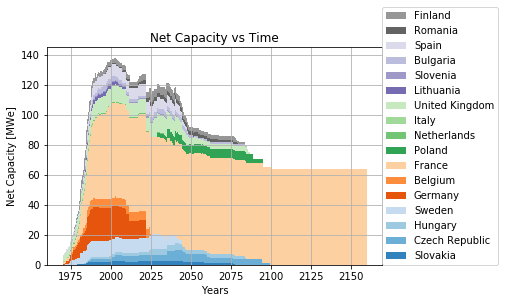
\includegraphics[width=\textwidth]{./onesim.png}
    \end{center}
    \caption{The simulated nuclear power deployment scheme. The historical operation of EU reactors is followed by the French transition to SFRs.  The steep transition from 2040 to 2060 reflects the scheduled decommissioning of reactors built in the 1975-2000 era of aggressive nuclear growth in France.}
    \label{fig:tot_dep}
\end{figure}


\end{document}
